\begin{frame}[fragile]{Assignments in Julia} \pause

\begin{columns}
  \begin{column}{0.45\textwidth}
    \centering
    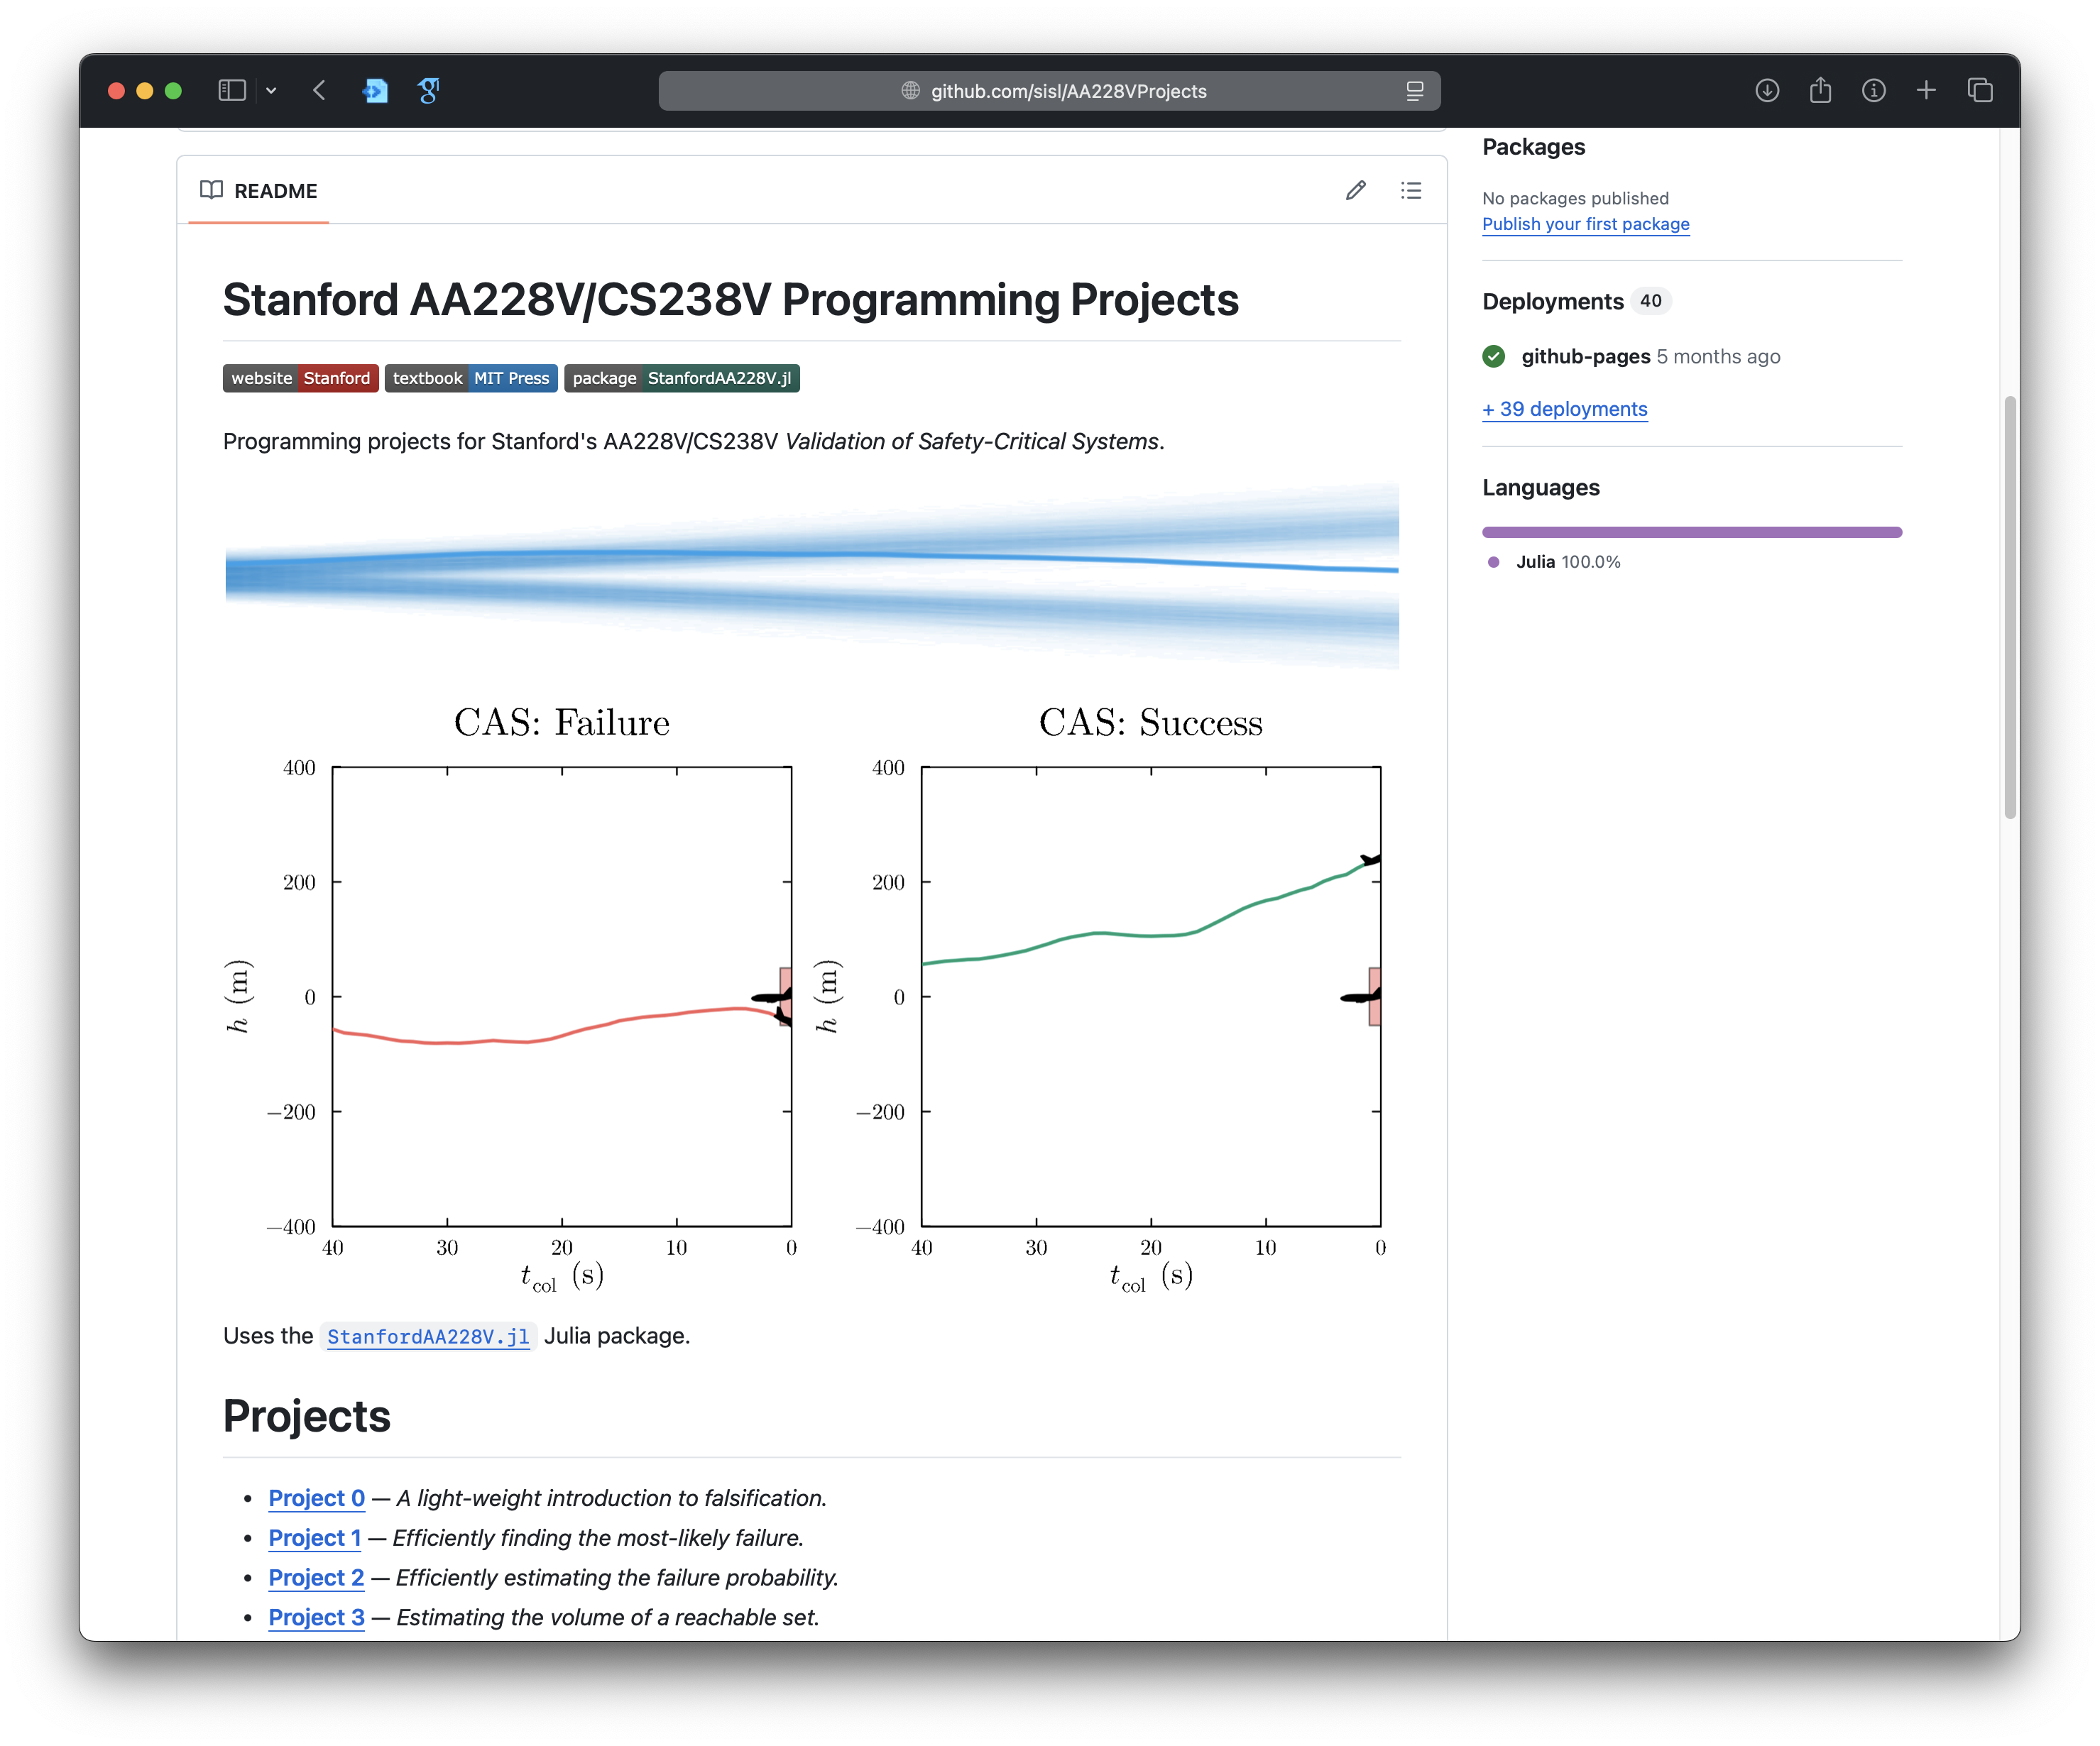
\includegraphics[width=\linewidth]{media/AA228VProjects.png}

    \captionof*{figure}{\shortstack{\footnotesize Assignments repository\\\textcolor{gray}{\scriptsize Student-facing code}}}
  \end{column}
  \pause
  \begin{column}{0.45\textwidth}
    \centering
    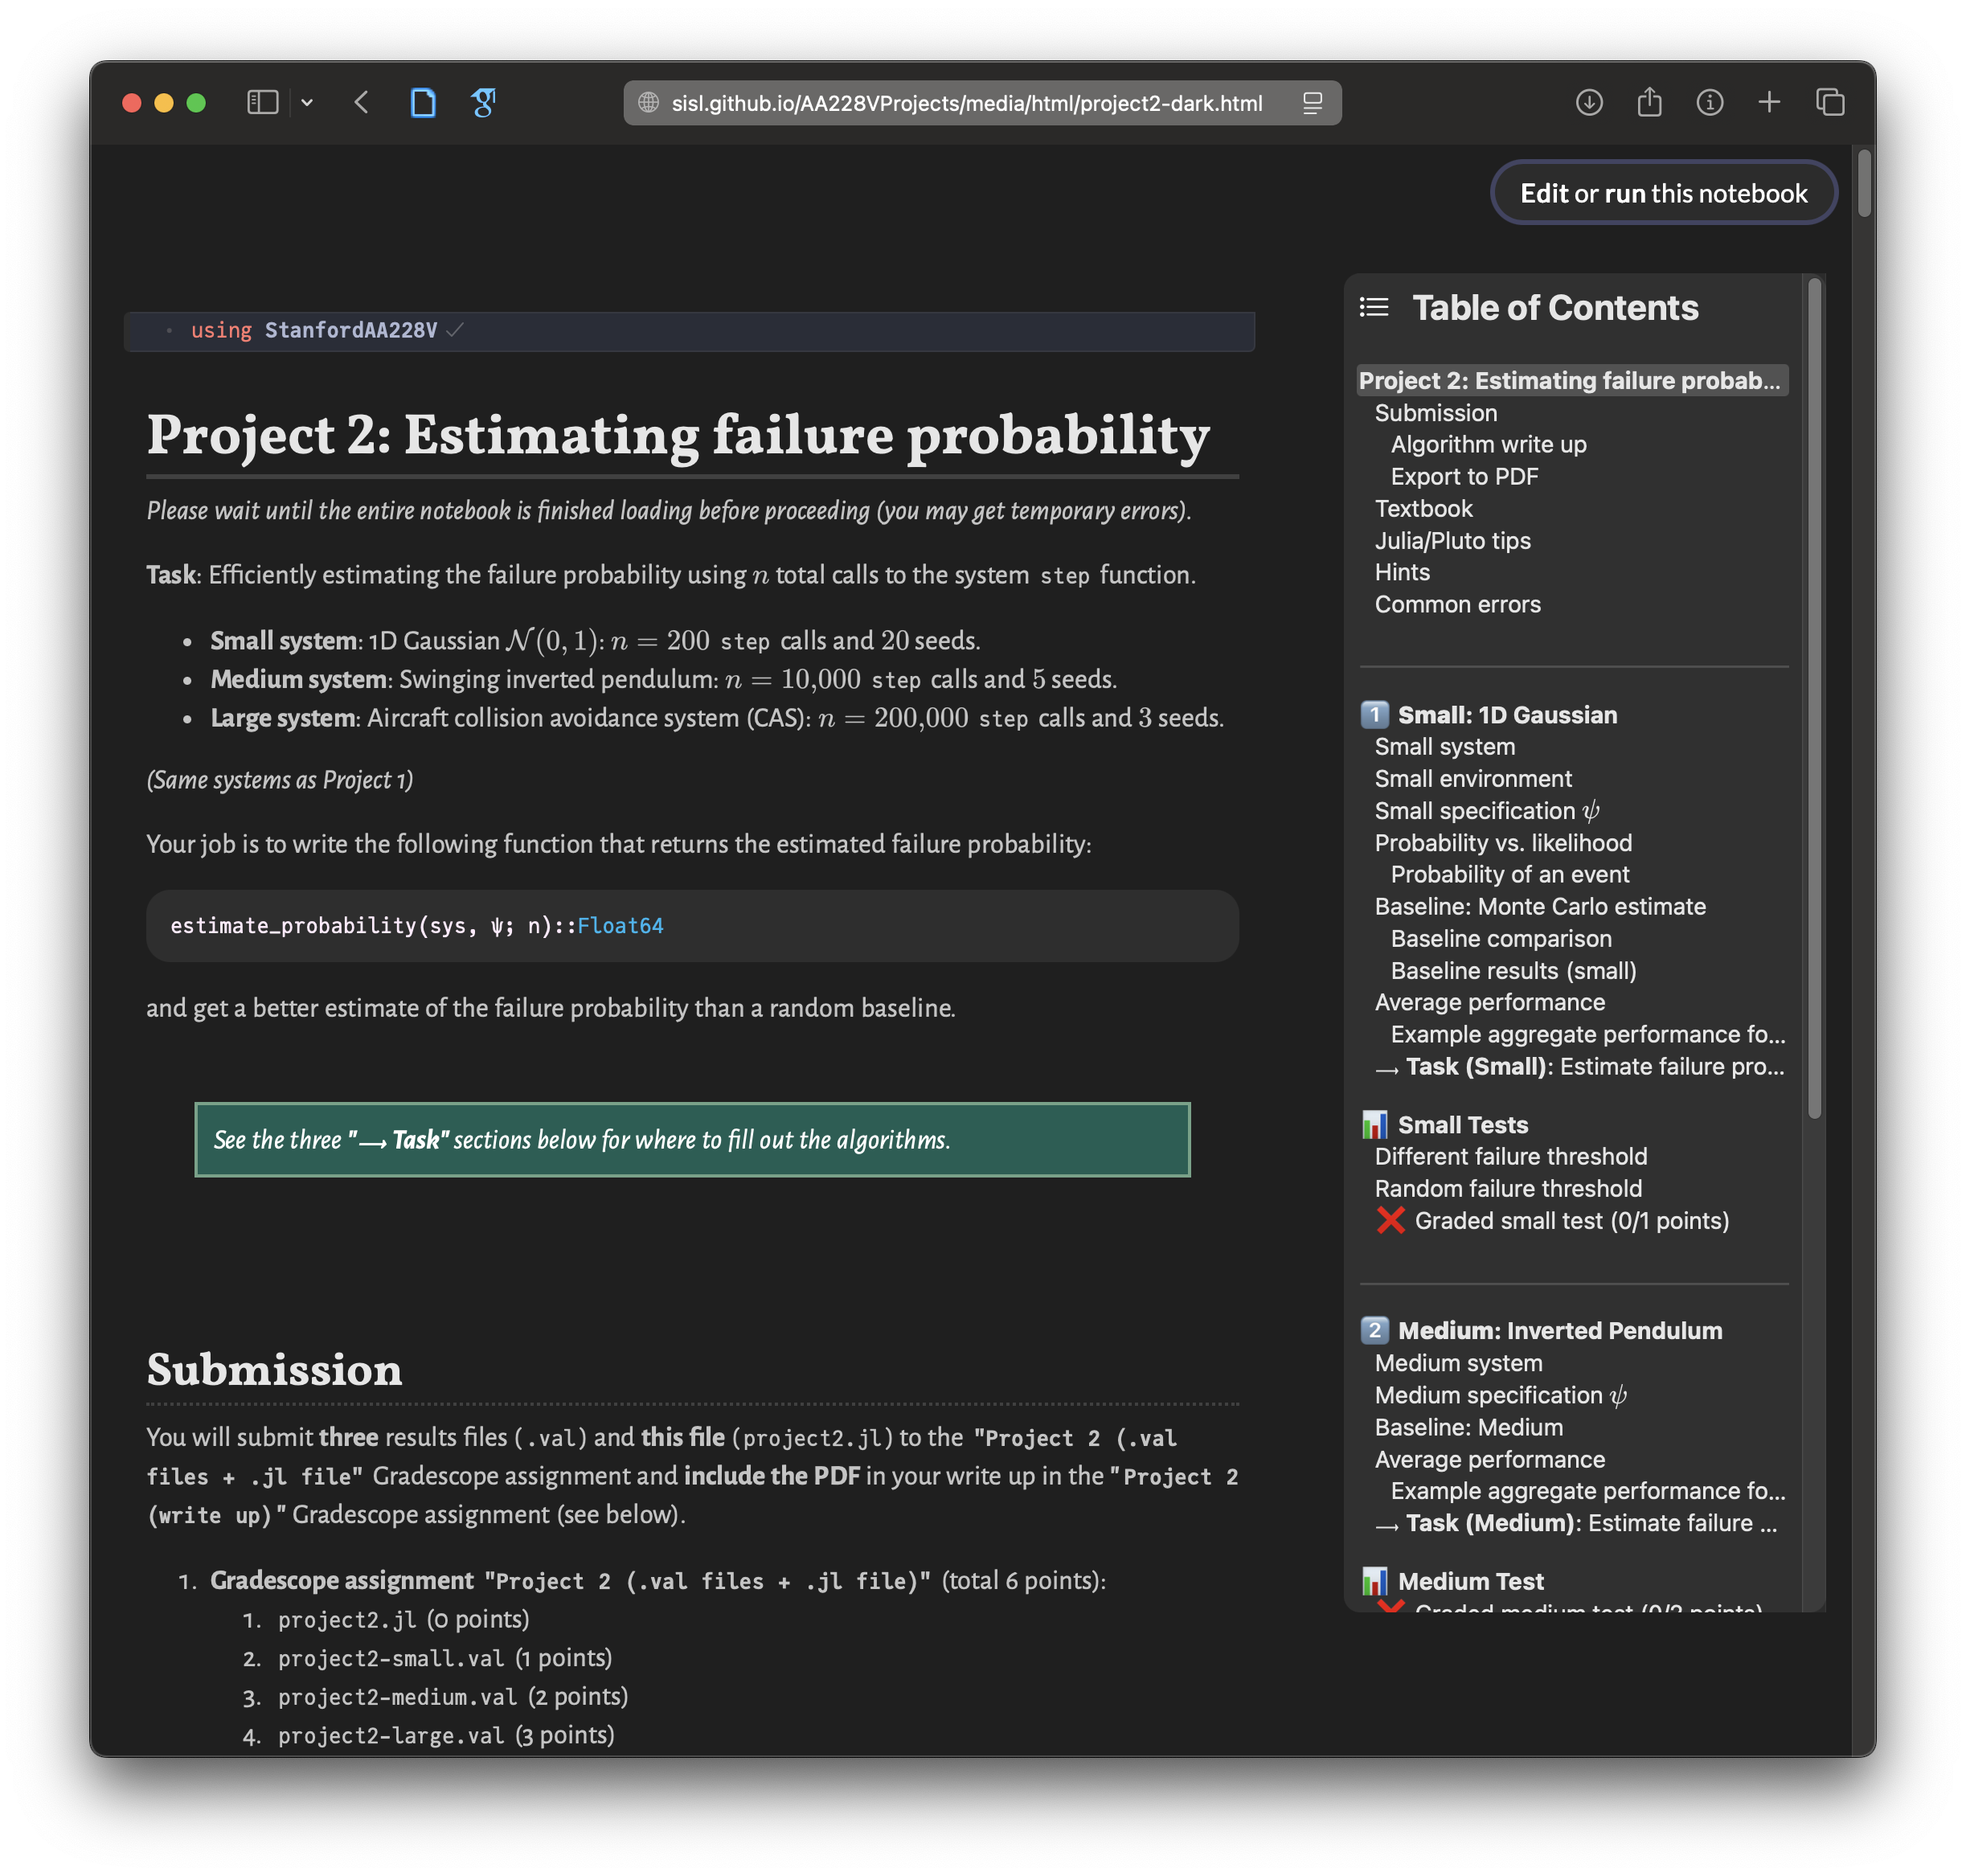
\includegraphics[width=\linewidth]{media/project2.png}

    \captionof*{figure}{\shortstack{\footnotesize Pluto assignments\\\textcolor{gray}{\scriptsize Includes local tests}}}
  \end{column}
  \hfill
\end{columns}

\end{frame}


\begin{frame}[fragile]{Assignments in Julia}

\begin{columns}
  \hfill
  \begin{column}{0.45\textwidth}
    \centering
    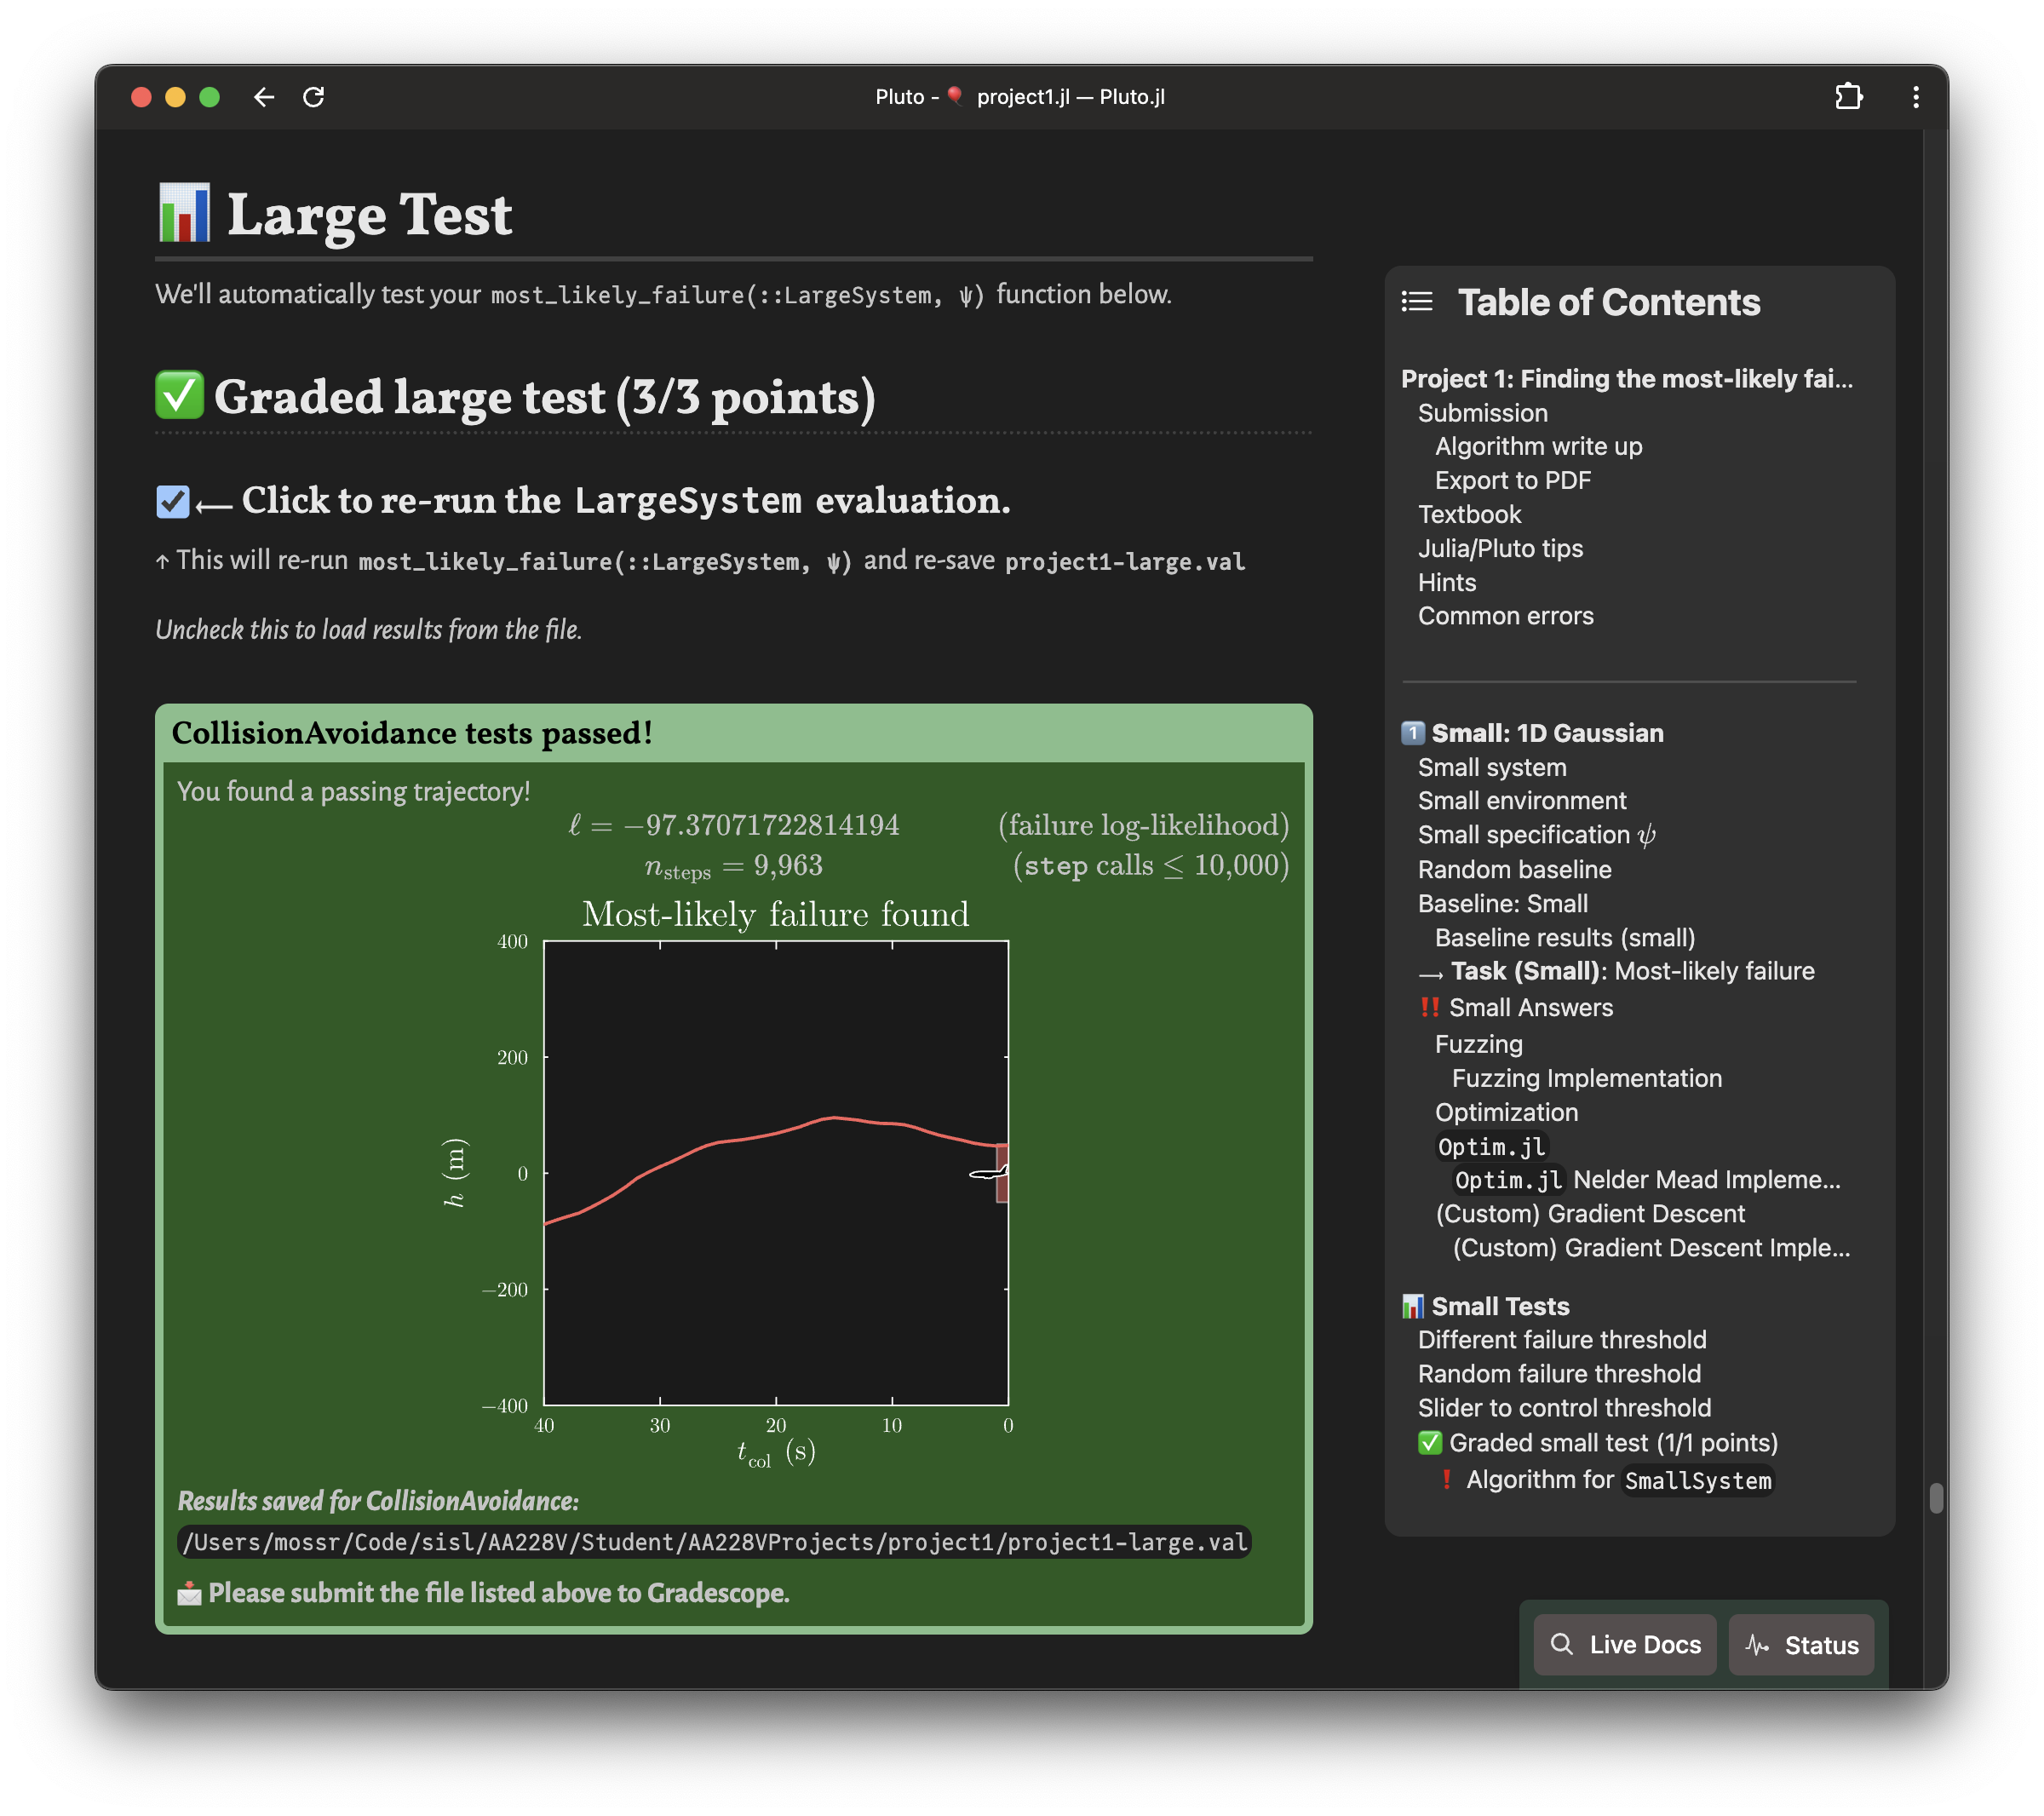
\includegraphics[width=\linewidth]{media/project1.png}

    \captionof*{figure}{\shortstack{\footnotesize Interactive Pluto assignments\\\textcolor{gray}{\scriptsize Get feedback instantly}}}
  \end{column}
  \pause
  \begin{column}{0.54\textwidth}
    \small
    \begin{itemize}
      \item Separated assignment code from core library (\jlv{StanfordAA228V.jl}) \pause
      \item Interactive nature allows students to play with their algorithms \pause
      \item No ``hidden state'' that may confuse students \pause
      \item Open-source nature requires clever obfuscation of solution code \pause
      \item Metaprogramming serves as lightweight way to track and enforce student requirements \pause
      \item Local tests exactly match graded tests \pause
    \end{itemize}
  \end{column}
  \hfill
\end{columns}

\end{frame}